\documentclass[aspectratio=169]{beamer}

%%%%%%%%%%%%%%%%%%%%%%%%%%%%%%%%%%%%%%%%%%%%%%%%%%%%%%%%%%%%%%%%%%%%%%%%%%%%%%%%%
% PREAMBLE

% DEFINE VARIABLES
\newcommand{\Lesson}{TEMA EJEMPLO}
\newcommand{\Subject}{Ejemplos, ejemplos, y ejemplos}
\newcommand{\Program}{Inversiones Financieras}
\newcommand{\Professor}{CUNEF Universidad}

% FOOTER WITH LOGO
\setbeamertemplate{footline}{
\hfill
\includegraphics[width=1.2cm]{figs/logo.png}\hspace{13cm}\vspace*{0.5cm}
\insertframenumber \hspace{1cm}
}

% FOOTER WITHOUT LOGO
\newcommand{\NoLogoFootline}{
    \setbeamertemplate{footline}{
    \hfill\vspace*{0.5cm}    
    }
}

% IDENTATION OPTIONS
\setlength{\leftmargini}{1em} % for itemize and enumerate level 1
\setlength{\leftmarginii}{1em} % for itemize and enumerate level 2
\setlength{\leftmarginiii}{1em} % for itemize and enumerate level 3

% PACKAGES
\usepackage{framed, color}
\definecolor{shadecolor}{rgb}{1,0.9,0.8}
\usepackage[absolute,overlay]{textpos}
\usepackage{graphicx, tikz,xcolor}
\usepackage{multirow, bigstrut,epstopdf}
\usepackage{amsmath,relsize,bigdelim}
\usepackage{hyperref}
\usepackage{tcolorbox}
\hypersetup{
    colorlinks=true,
    linkcolor=blue,
    filecolor=magenta,      
    urlcolor=cyan,
}
\usepackage[font=tiny]{caption}

% COLOR OPTIONS
\definecolor{CUNEFOrange}{RGB}{255, 87, 0}
\definecolor{CUNEFGray}{RGB}{214, 209, 196}
\definecolor{Front}{RGB}{21,31,108}
% BEAMER OPTIONS
\setbeamertemplate{navigation symbols}{}
\setbeamercolor{itemize item}{fg = CUNEFOrange}
\setbeamercolor{itemize subitem}{fg = CUNEFOrange}
\setbeamercolor{itemize subsubitem}{fg = CUNEFOrange}		
\setbeamercolor{enumerate item}{fg = CUNEFOrange}
\setbeamercolor{enumerate subitem}{fg = CUNEFOrange}
\setbeamercolor{enumerate subsubitem}{fg = CUNEFOrange}		
\setbeamercolor{normal text}{fg=Front}

\setbeamercolor{frametitle}{fg=CUNEFOrange}


% NEW TITLE SLIDE
\newcommand{\CUNEFTitleSlide}{\begin{frame}

%\begin{textblock*}{0.1\paperwidth}(0.01\paperwidth,0.01\paperwidth)
%\includegraphics[width=0.3\paperwidth]{Logo_WQU.png}
%\end{textblock*}

\vspace{2em}
%\centering\scriptsize{{\textcolor{CUNEFOrange}{\Lesson}}} \\[1em]
\centering\textbf{{\large\textcolor{CUNEFOrange}{Econometrics 2024/2025}}} \\ [1em]
\centering{\large\textcolor{CUNEFOrange}{}} \\ [1em]
\vspace{0.5em}
\centering{\normalsize\textcolor{CUNEFOrange}{Multiple Regression Analysis: Inference}}
\end{frame}}

% NEW SLIDE TEMPLATE
\newcommand{\slide}[2]{\begin{frame}
%\begin{textblock*}{0.1\paperwidth}(0.01\paperwidth,0.01\paperwidth)
%\includegraphics[width=0.15\paperwidth]{Logo_WQU.png}
%\end{textblock*}


\begin{textblock*}{0.87\paperwidth}(0.05\paperwidth,1.2cm)
{\Large\textcolor{CUNEFOrange}{#1}}
\end{textblock*}

\begin{textblock*}{0.87\paperwidth}(0.05\paperwidth,2cm)
#2
\end{textblock*}

\begin{textblock*}{\paperwidth}(0.01\paperwidth,0.95\paperheight)
\noindent\begin{tikzpicture}
%\draw[CUNEFOrange] (0,0) rectangle (0.9\paperwidth,0.8em);
%\draw[CUNEFOrange] (0.9\paperwidth+0.01\paperwidth,0) rectangle (\paperwidth-0.02\paperwidth,0.8em);
%\node[right] at (0,0.4em) {\tiny\textcolor{CUNEFGray}{\Subject\enspace-- \Program\enspace-- \Professor\enspace}};
\end{tikzpicture}
{\tiny\textcolor{CUNEFGray}\thepage}
\end{textblock*}
\end{frame}
}
%%%%%%%%%%%%%%%%%%%%%%%%%%%%%%%%%%%%%%%%%%%%%%%%%%%%%%%%%%%%%%%%%%%%%%%%%%%%%%%%%
% TOC AT BEGINNING OF EACH SECTION
\AtBeginSection[]{
    \begin{frame}<beamer>
    \frametitle{\textcolor{CUNEFOrange}{Outline}}
    \tableofcontents[currentsection]
    \end{frame}
}


\begin{document}

%%%%%%%%%%%%%%%%%%%%%
% Title Page
%%%%%%%%%%%%%%%%%%%%
\NoLogoFootline
{\usebackgroundtemplate{%
  
\includegraphics[width=\paperwidth,height=\paperheight]{figs/title_page.png}}
\CUNEFTitleSlide}


\setbeamertemplate{footline}{
\hfill
\includegraphics[width=1.2cm]{figs/logo.png}\hspace{13cm}\vspace*{0.5cm}
\insertframenumber \hspace{1cm}
}

\begin{frame}
\frametitle{\textcolor{CUNEFOrange}{Outline}}
   \tableofcontents 
\end{frame}

\frame<beamer>{\frametitle{\textcolor{CUNEFOrange}{Multiple Regression Analysis: Inference}}

\begin{itemize}
\item Statistical inference in the regression model
\begin{itemize}
\item Hypothesis tests about population parameters
\item Construction of confidence intervals 
\end{itemize}
\item Sampling distributions of the OLS estimators
 \begin{itemize}
\item The OLS estimators are random variables
\item We already know their expected values and their variances
\item However, for hypothesis tests we need to know their distribution
\item In order to derive their distribution we need additional assumptions
\item Assumption about distribution of errors: normal distribution
\end{itemize}
\end{itemize}
}

\section{Sampling Distributions of the OLS Estimators}
\frame<beamer>{\frametitle{\textcolor{CUNEFOrange}{Assumption MLR.6 (Normality of error terms) }}
$u_i \sim \text{Normal}(0,\sigma^2)$ independently of $x_{i1}, x_{i2}, \ldots, x_{ik}$
\noindent
\begin{minipage}{.45\textwidth}
   \begin{figure}[htp]
    %\centering
    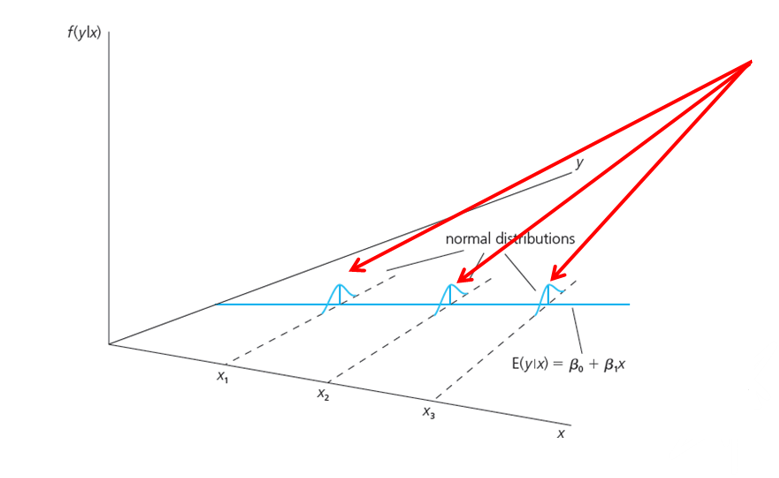
\includegraphics[width=1\textwidth]{figs/normality.png}
 \end{figure}
\end{minipage}%
\hspace{1cm} 
\begin{minipage}{.45\textwidth}
\vspace{0.5cm}
\begin{itemize}
    \item It is assumed that the unobserved factors are normally distributed around the population regression function

\item The form and the variance of the distribution does not depend on any of the explanatory variables


\end{itemize} 

\end{minipage}
It follows that:
\[ y|\mathbf{x} \sim \text{Normal}(\beta_0 + \beta_1 x_1 +\ldots + \beta_k x_k, \sigma^2) \]
}


\frame<beamer>{\frametitle{\textcolor{CUNEFOrange}{Discussion of the normality assumption}}

\begin{itemize}
    \item The error term is the sum of “many” different unobserved factors.
\item Sums of independent factors are normally distributed (CLT).
\item Problems:
\begin{itemize}
    \item How many different factors? Number large enough?
   \item Possibly very heterogenuous distributions of individual factors
   \item How independent are the different factors?
\end{itemize} 
\item The normality of the error term is an empirical question.
\item At least, the error distribution should be “close” to normal.
\item In many cases, normality is questionable or impossible by definition.

\end{itemize} 

}

\frame<beamer>{\frametitle{\textcolor{CUNEFOrange}{Discussion of the normality assumption (cont.)}}

\begin{itemize}
\item Examples where normality cannot hold:
\begin{itemize}
    \item Wages (nonnegative; also: minimum wage)
    \item Number of arrests (takes on a small number of integer values)
    \item Unemployment (indicator variable, takes on only 1 or 0)
\end{itemize} 
\item In some cases, normality can be achieved through transformations    of the dependent variable (e.g. use log(wage) instead of wage).
\item Under normality, OLS is the best (even nonlinear) unbiased estimator
\item Important: For the purposes of statistical inference, the assumption   of normality can be replaced by a large sample size.


\end{itemize} 

}

\frame<beamer>{\frametitle{\textcolor{CUNEFOrange}{Terminology}}
\begin{itemize}
    \item MLR.1 - MLR.5 are "Gauss-Markov assumptions"
    \item MLR.1 - MLR.6 are "Classical linear model (CLM) assumptions"
    \item Theorem 4.1 (Normal sampling distributions)
    \item Under assumptions MLR.1 – MLR.6:
\begin{itemize}
        \item The estimators are normally distributed around the true parameters with the variance that was derived earlier 
\[\hat \beta_j \sim \text{Normal}(\beta_j, \text{Var}(\hat \beta_j ))
\]
        \item The standazed estimators follow a standard normal distribution
\[ \frac{\hat \beta_j- \beta_j}{\text{sd}(\hat \beta_j)} \sim \text{Normal}(0,1)
\]
    \end{itemize}

\end{itemize} 


}


\frame<beamer>{\frametitle{\textcolor{CUNEFOrange}{Testing hypotheses about a single population parameter}}
\begin{itemize}
    \item Theorem 4.2 (t-distribution for the standardized estimators)
    \item Under assumptions MLR.1 – MLR.6:
\begin{itemize}
        \item If the standardization is done using the \underline{estimated} standard deviation (= standard error), the normal distribution is replaced by a t-distribution
\[ \frac{\hat \beta_j- \beta_j}{\text{sd}(\hat \beta_j)} \sim \text{t}_{(n-k-1)}
\]
Note: the t-distribution is close to the standard normal if $n-k-1$ is large.
    \end{itemize}
     \item Null hypothesis (for more general hypotheses, see below)
\[H_0~:~\beta_j = 0
\]
The population parameter is equal to zero, i.e. after controlling for the other independent variables, there is no effect of $x_j$ in $y$
\end{itemize} 

}

\section{Testing Hypotheses about a Single Population
Parameter: The t-test}
\frame<beamer>{\frametitle{\textcolor{CUNEFOrange}{t-statistic (or t-ratio)
}}
\[ t_{\hat \beta_j} \equiv \frac{\hat \beta_j}{\text{se}(\hat \beta_j)}\]
\begin{itemize}
\item The t-statistic will be used to test the above null hypothesis. The farther the estimated coefficient is from zero, the less likely is that the null hypothesis holds true. But what does "far" away from zero mean?
\item This depends on the variability of the estimated coefficient, i.e. its standard deviation. \textbf{The t-statistic measures how many estimated standard deviations the estimated coefficient is away from zero}
\item Distribution of the t-statistic if the null hypothesis is true
\[ t_{\hat \beta_j} \equiv \hat \beta_j/\text{se}(\hat \beta_j)=(\hat \beta_j- \beta_j)/\text{se}(\hat \beta_j) \sim t_{n-k-1}\]
\item Goal: Define a rejection rule so that, if it is true, $H_0$ is rejected only with a small probability (= significance level, e.g. 5\%)

\end{itemize}
}

\frame<beamer>{\frametitle{\textcolor{CUNEFOrange}{Testing against one-sided alternatives (greater than zero)
 }}
\noindent
\begin{minipage}{.45\textwidth}
   \begin{figure}[htp]
    %\centering
    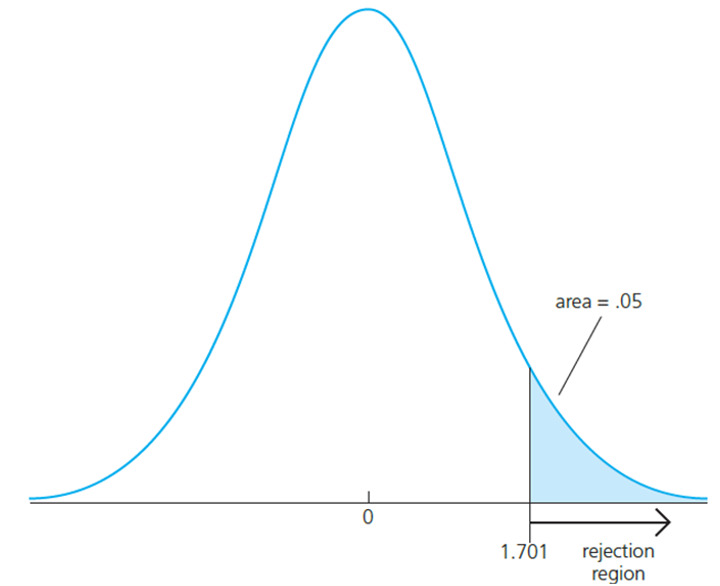
\includegraphics[width=1\textwidth]{figs/norm_test.png}
 \end{figure}
\end{minipage}%
\hspace{1cm} 
\begin{minipage}{.45\textwidth}
\vspace{0.5cm}
\begin{itemize}
    \item Reject the null hypothesis in favour of the alternative hypothesis if the estimated coefficient is \underline{too large} (i.e. larger than a critical value).

\item Construct the critical value so that, if the null hypothesis is true, it is rejected in, for example, 5\% of the cases.

\item In the given example, this is the point of the t-distribution with 28 degrees of freedom that is exceeded in 5\% of the cases.

\item Reject if t-statistic is greater than $1.701$

\end{itemize} 

\end{minipage}

}

\frame<beamer>{\frametitle{\textcolor{CUNEFOrange}{Example: Wage equation
 }}
\begin{itemize}
    \item Test whether, after controlling for education and tenure, higher work experience leads to higher hourly wages.

\begin{figure}[htp]
    %\centering
    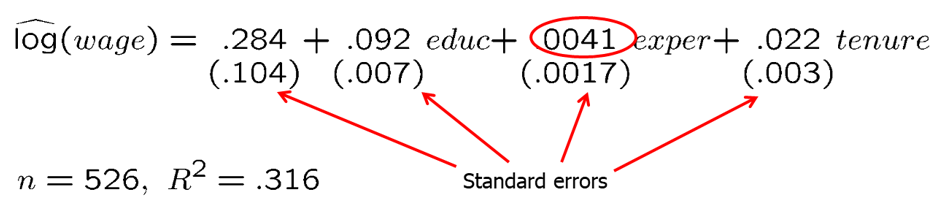
\includegraphics[width=0.8\textwidth]{figs/example_wage.png}
 \end{figure}
\item Test $H_0:~\beta_{exper} = 0$ against $H_1:~\beta_{exper} > 0$.
\item One would either expect a positive effect of experince on hourly wage or no effect at all.  
\end{itemize} 
}

\frame<beamer>{\frametitle{\textcolor{CUNEFOrange}{Example: Wage equation (cont.)
 }}
\begin{itemize}
    \item $t_{exper} = .0041/.0017 \approx 2.41$ $\leftarrow$ t-statistic
\item $df = n-k-1=526-3-1=522$ $\leftarrow$  Degrees of freedom; Here the standard normal approximation applies
\item $c_{0.05}= 1.645 $
\item $c_{0.01}= 2.326 $
\item Critical values for the 5\% and the 1\% significance level (these are conventional significance levels). 
\item  The null hypothesis is rejected because the t-statistic exceeds the critical value
\end{itemize} 
$\Rightarrow$ The effect of experience on hourly wage is statistically greater than zero at the 5\% (and even at the 1\%) significance level.

}

\frame<beamer>{\frametitle{\textcolor{CUNEFOrange}{Testing against one-sided alternatives (less than zero)
 }}
\noindent
\begin{minipage}{.45\textwidth}
   \begin{figure}[htp]
    %\centering
    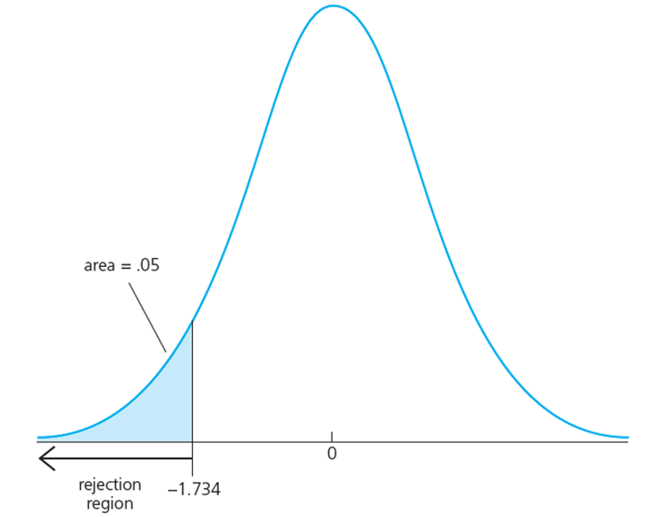
\includegraphics[width=1\textwidth]{figs/norm_test_right.png}
 \end{figure}
\end{minipage}%
\hspace{1cm} 
\begin{minipage}{.45\textwidth}
\vspace{0.5cm}
\begin{itemize}
    \item Reject the null hypothesis in favour of the alternative hypothesis if the estimated coefficient is \underline{too small} (i.e. smaller than a critical value).

\item Construct the critical value so that, if the null hypothesis is true, it is rejected in, for example, 5\% of the cases.

\item In the given example, this is the point of the t-distribution with 18 degrees of freedom so that 5\% of the cases are below the point.

\item Reject if t-statistic is less than -1.734


\end{itemize} 

\end{minipage}

}

\frame<beamer>{\frametitle{\textcolor{CUNEFOrange}{Example: Student performance and school size }}
Test whether smaller school size leads to better student performance

\begin{figure}[htp]
    %\centering
    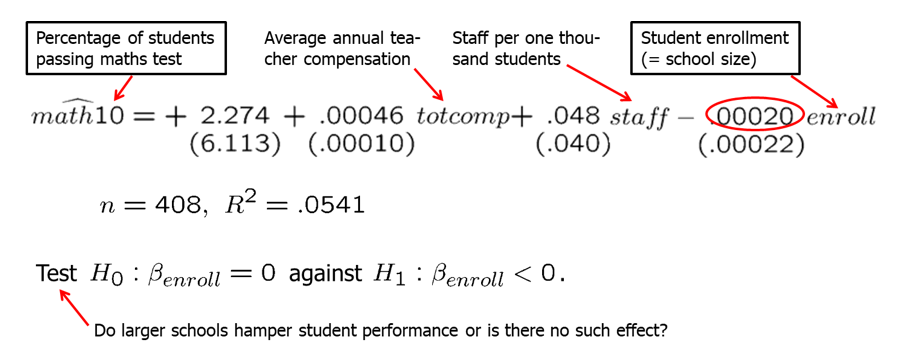
\includegraphics[width=0.9\textwidth]{figs/wage equation2.png}
 \end{figure}

}

\frame<beamer>{\frametitle{\textcolor{CUNEFOrange}{Example: Student performance and school size (cont.)}}
Test whether smaller school size leads to better student performance

\begin{figure}[htp]
    %\centering
    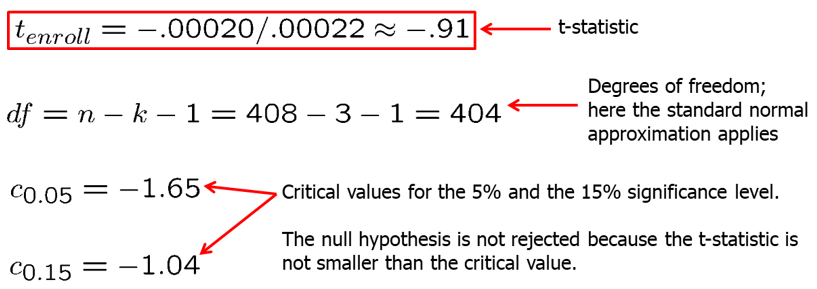
\includegraphics[width=0.9\textwidth]{figs/wage equation3.png}
 \end{figure}
$\Rightarrow$ One cannot reject the hypothesis that there is no effect of school size on student performance (not even for a lax significance level of 15\%).

}

\frame<beamer>{\frametitle{\textcolor{CUNEFOrange}{Example: Student performance and school size (cont.)}}
Alternative specification of functional form:

\begin{figure}[htp]
    %\centering
    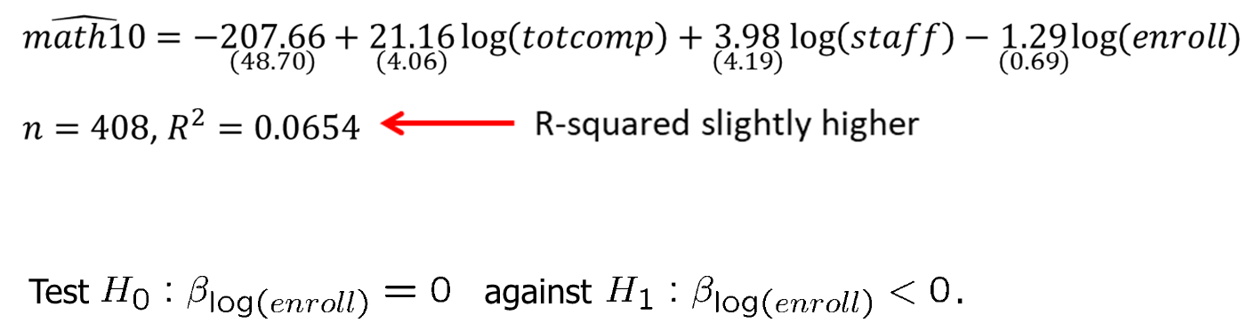
\includegraphics[width=0.9\textwidth]{figs/wage equation4.png}
 \end{figure}

}

\frame<beamer>{\frametitle{\textcolor{CUNEFOrange}{Example: Student performance and school size (cont.)
 }}
\begin{itemize}
    \item$t_{\text{log}(enroll)}= -1.29/.69 \approx -1.89$ $\leftarrow$ t-statistic
\item $c_{0.05} = -1.65$ $\leftarrow$ Critical value for 5\% significance level; reject the null hypothesis
\item The hypothesis that there is no effect of school size on student performance can be rejected in favor of the hypothesis that the effect is negative.
\item How large is the effect?
\[
-1.29 = \frac{\Delta \widehat{math10}}{\Delta \text{log}(enroll)}= \frac{\Delta \widehat{math10}}{\frac{\Delta (enroll)}{enroll}}=\frac{\frac{-1.29}{100}}{\frac{1}{100}}=\frac{-0.0129}{+1\%}
\]
$\Rightarrow$ $+ 1\%$ enrollment; -0.129 percentage points students pass test
\end{itemize} 

}

\frame<beamer>{\frametitle{\textcolor{CUNEFOrange}{Testing against two-sided alternatives
 }}
\noindent
\begin{minipage}{.45\textwidth}
   \begin{figure}[htp]
    %\centering
    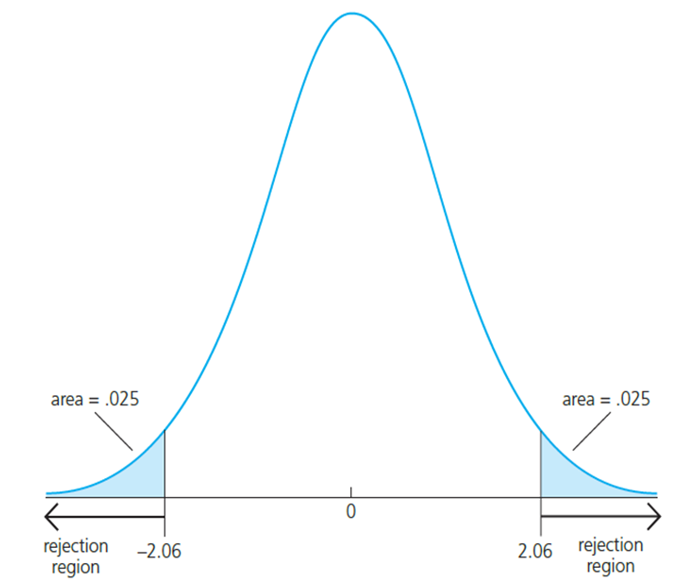
\includegraphics[width=1\textwidth]{figs/norm_test_two.png}
 \end{figure}
\end{minipage}%
\hspace{1cm} 
\begin{minipage}{.45\textwidth}
\vspace{0.5cm}
\begin{itemize}
    \item Reject the null hypothesis in favour of the alternative hypothesis if the absolute value of the estimated coefficient is too large.

\item Construct the critical value so that, if the null hypothesis is true, it is rejected in, for example, 5\% of the cases.

\item In the given example, these are the points of the t-distribution so that 5\% of the cases lie in the two tails.

\item Reject if absolute value of t-statistic is less than -2.06 or greater than 2.06



\end{itemize} 

\end{minipage}

}

\frame<beamer>{\frametitle{\textcolor{CUNEFOrange}{Example: Determinants of college GPA
 }}
\begin{figure}[htp]
    %\centering
    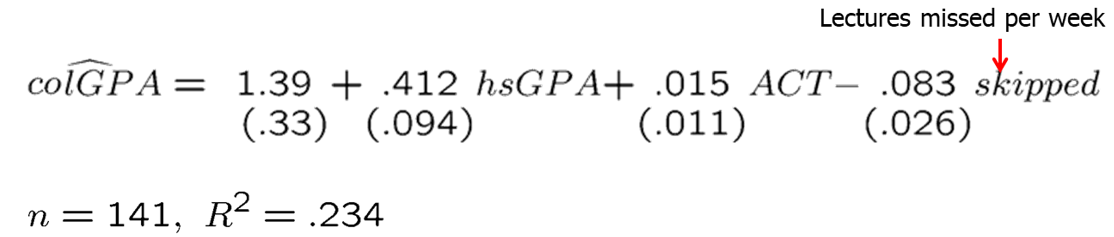
\includegraphics[width=0.9\textwidth]{figs/lectures.png}
 \end{figure}
\begin{itemize}
    \item $t_{hsGPA}=4.38 > c_{0.01}=2.58$
\item $t_{ACT}=1.36 < c_{0.10}=1.645$
\item $|t_{skipped}| = |-3.19| > c_{0.01} = 2.58$

\end{itemize} 
$\Rightarrow$ The effects of hsGPA and skipped are significantly different from zero at the 1\% significance level. The effect of ACT is not significantly different from zero,  not even at the 10\% significance level.
}

\frame<beamer>{\frametitle{\textcolor{CUNEFOrange}{``Statistically significant'' variables in a regression }}
\begin{itemize}
    \item If a regression coefficient is different from zero in a two-sided test, the corresponding variable is said to be ``statistically significant''.
	\item If the number of degrees of freedom is large enough so that the normal approximation applies, the following rules of thumb apply:
\end{itemize} 
\begin{tcolorbox}[colback=white,colframe=CUNEFOrange]
$|t-ratio| > 1.645$ $\rightarrow$ ``statistically significant at 10\%level''\\

$|t-ratio| > 1.96$ $\rightarrow$ ``statistically significant at 5\%level''\\

$|t-ratio| > 2.576$ $\rightarrow$ ``statistically significant at 1\%level''\\
\end{tcolorbox}
}

\frame<beamer>{\frametitle{\textcolor{CUNEFOrange}{Example: Campus crime and enrollment }}
\begin{itemize}
    \item An interesting hypothesis is whether crime increases by one percent if enrollment is increased by one percent.
 
\end{itemize}
\begin{figure}[htp]
    %\centering
    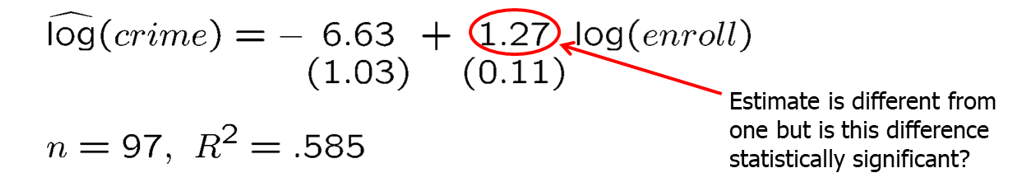
\includegraphics[width=0.8\textwidth]{figs/crime.png}
\end{figure}
\begin{itemize}
    \item $H_0:~\beta_{\text{log}(enroll)}=1$, $H_0:~\beta_{\text{log}(enroll)}\neq 1$
 \item $t = \frac{1.27-1}{.11} \approx 2.45>1.985=c_{0.05}$
\item[$\rightarrow$] The hypothesis is rejected at the 5\% level
\end{itemize}
}

\frame<beamer>{\frametitle{\textcolor{CUNEFOrange}{Computing p-values for t-tests }}
\begin{itemize}
    \item If the significance level is made smaller and smaller, there will be a point where the null hypothesis cannot be rejected anymore.
\item The reason is that, by lowering the significance level, one wants to avoid more and more to make the error of rejecting a correct $H_0$.
\item The smallest significance level at which the null hypothesis is still rejected, is called the p-value of the hypothesis test.
\item A small p-value is evidence against the null hypothesis because one would reject the null hypothesis even at small significance levels.
\item A large p-value is evidence in favor of the null hypothesis.
\item P-values are more informative than tests at fixed significance levels.

\end{itemize}

}

\frame<beamer>{\frametitle{\textcolor{CUNEFOrange}{How the p-value is computed (here: two-sided test)? }}
\noindent
\begin{minipage}{.45\textwidth}
%\vspace{-1cm}
   \begin{figure}[h]
    %\centering
    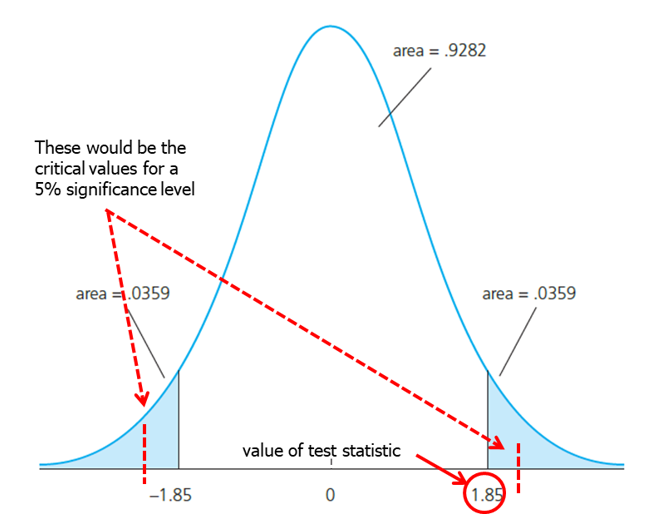
\includegraphics[width=1\textwidth]{figs/pvalue.png}
 \end{figure}
\begin{itemize}
    \item The p-value is the significance level at which one is indifferent between rejecting and not rejecting the null hypothesis. 
\end{itemize}
\end{minipage}%
\hspace{1cm} 
\begin{minipage}{.45\textwidth}
\vspace{0.5cm}

\begin{itemize}
\item In the two-sided case, the p-value is thus the probability that the t-distributed variable takes on a larger absolute value than the realized value of the test statistic, e.g.

		$P(|t|>1.85) = 2*(0.0359) = .0718$

\item From this, it is clear that a null hypothesis is rejected if and only if the corresponding p-value is smaller than the significance level.

\item For example, for a significance level of 5\% the t-statistic would not lie in the rejection region.
\end{itemize} 
\end{minipage}
}

\frame<beamer>{\frametitle{\textcolor{CUNEFOrange}{Guidelines for discussing economic and statistical significance
}}
\begin{itemize}
    \item If a variable is statistically significant, discuss the magnitude of the coefficient to get an idea of its economic or practical importance.
\item The fact that a coefficient is statistically significant does not necessarily mean it is economically or practically significant!
\item If a variable is statistically and economically important but has the ``wrong'' sign, the regression model might be misspecified.
\item If a variable is statistically insignificant at the usual levels (10\%, 5\%, or 1\%), one may think of dropping it from the regression.
\item If the sample size is small, effects might be imprecisely estimated so that the case for dropping insignificant variables is less strong.

\end{itemize}

}

\section{Confidence intervals}
\frame<beamer>{\frametitle{\textcolor{CUNEFOrange}{Confidence intervals }}
\begin{itemize}
    \item Simple manipulation of the result in Theorem 4.2 implies that
\begin{figure}[htp]
    %\centering
    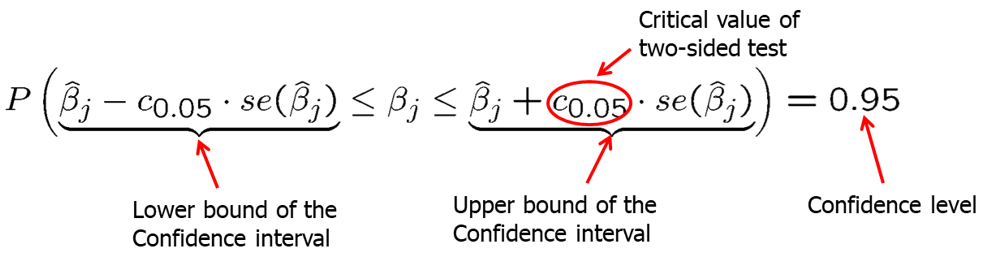
\includegraphics[width=0.8\textwidth]{figs/ci.png}
\end{figure}
\item Interpretation of the confidence interval
 \begin{itemize}
    \item The bounds of the interval are random.
\item In repeated samples, the interval that is constructed in the above way will cover the population regression coefficient in 95\% of the cases.
\end{itemize}
\end{itemize}

}

\frame<beamer>{\frametitle{\textcolor{CUNEFOrange}{Confidence intervals for typical confidence levels
 }}
\begin{tcolorbox}[colback=white,colframe=CUNEFOrange]
$P(\hat \beta_j - c_{0.01}\cdot se(\hat \beta_j)\leq \beta_j \leq \hat \beta_j + c_{0.01}\cdot se(\hat \beta_j)) = 0.99$ \\

$P(\hat \beta_j - c_{0.05}\cdot se(\hat \beta_j)\leq \beta_j \leq \hat \beta_j + c_{0.01}\cdot se(\hat \beta_j)) = 0.95$ \\

$P(\hat \beta_j - c_{0.10}\cdot se(\hat \beta_j)\leq \beta_j \leq \hat \beta_j + c_{0.01}\cdot se(\hat \beta_j)) = 0.90$ \\
\end{tcolorbox}
\begin{itemize}
    \item Relationship between confidence intervals and hypotheses tests
\[
a_j \notin interval \Rightarrow \text{reject } H_0:~\beta_j = \alpha_j \text{ in favor of } H_1:~\beta_j \neq \alpha_j
\]
\end{itemize}

}

\frame<beamer>{\frametitle{\textcolor{CUNEFOrange}{Example: Model of firms' R\&D expenditures
 }}
\begin{figure}[htp]
    %\centering
    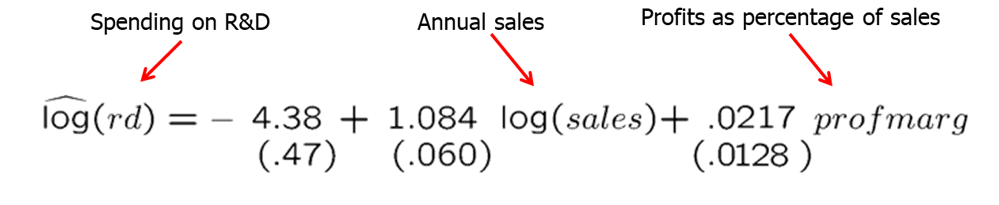
\includegraphics[width=0.8\textwidth]{figs/randd.png}
\end{figure}
\begin{itemize}
    \item $n=23$, $R^2=.918$, $df=32-2-1=29$ $\Rightarrow$ $c_{0.05}=2.045$
\item The confidence interval for the effect of sales on R\&D is $1.084 \pm 2.045\cdot (.060)= [.961, 1.21]$.
\item[$\rightarrow$] The effect of sales on R\&D is relatively precisely estimated as the interval is narrow. Moreover, the effect is significantly different from zero because zero is outside of the interval.
\item The confidence interval for the effect of the profit as percentage of sales on R\&D is $.0217 \pm 2.045\cdot (.02118)= [-.0045, .0479]$.
\item[$\rightarrow$] The effect is imprecisely estimated as the interval is very wide. It is not even statistically significant as the zero lies in the interval.
\end{itemize}

}
\section{Testing hypotheses about a linear combination of the parameters}
\frame<beamer>{\frametitle{\textcolor{CUNEFOrange}{Testing hypotheses about a linear combination of the parameters
 }}
\begin{itemize}
    \item Example: Return to education at two-year vs. at four-year colleges
\begin{figure}[htp]
    %\centering
    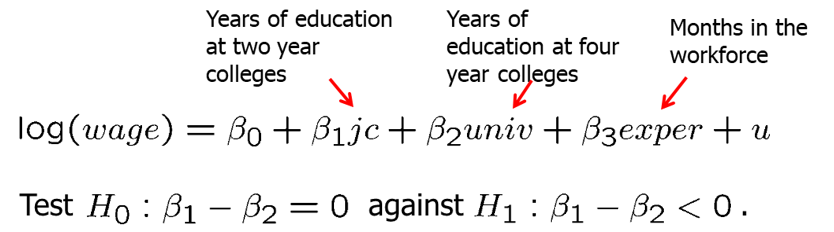
\includegraphics[width=0.7\textwidth]{figs/wage.png}
\end{figure}
\item Test $H_0:~\beta_1-\beta_2 = 0$ against $H_1:~\beta_1-\beta_2 < 0$
\item A possible test statistic would be: $t=\frac{\hat\beta_1-\hat\beta_2}{se(\hat\beta_1-\hat\beta_2)}$
\item The difference between the estimates is normalized by the estimated standard deviation of the difference. The null hypothesis would have to be rejected if the statistic is ``too negative'' to believe that the true difference between the parameters is equal to zero
\end{itemize}

}

\frame<beamer>{\frametitle{\textcolor{CUNEFOrange}{Testing hypotheses about a linear combination of the parameters (cont.)
 }}
\begin{itemize}
    \item The standard error of the difference in parameters is impossible to obtain with standard regression output\\
$se(\hat\beta_1-\hat\beta_2) = \sqrt{\text{Var}(\hat\beta_1-\hat\beta_2)}=\sqrt{\text{Var}(\hat\beta_1)+\text{Var}(\hat\beta_2)+2\text{Cov}(\hat\beta_1,\hat\beta_2)}$

\item[$\rightarrow$] $\text{Cov}(\hat\beta_1,\hat\beta_2)$ is usually not available in regression output
\item An alternative method is to make a substitution in variables:\\
Define $\theta_1=\beta_1-\beta_2$ and test $H_0:~\theta_1=0$ against $H_1:~\theta_1<0$
\begin{figure}[htp]
    %\centering
    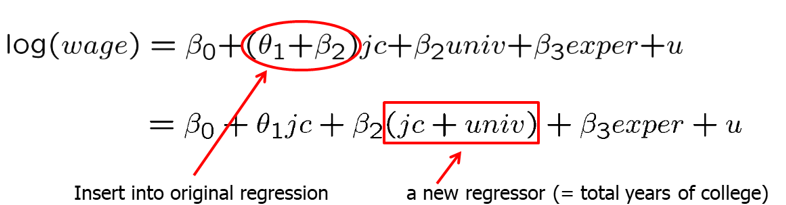
\includegraphics[width=0.8\textwidth]{figs/subst.png}
\end{figure}
\end{itemize}

}

\frame<beamer>{\frametitle{\textcolor{CUNEFOrange}{Estimation results}}
\begin{figure}[htp]
    %\centering
    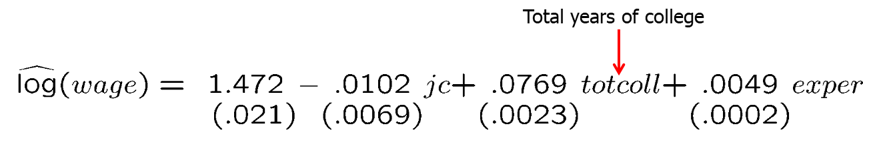
\includegraphics[width=0.8\textwidth]{figs/totcoll.png}
\end{figure}
\begin{itemize}
    \item $n=6 763$, $R^2=.222$
\item $t=-.0102/.0069=-1.48$
\item $p-value = P(t-ratio<-1.48)=.070$
\item $CI = -.0102 \pm 1.96(.0069)=[-.0237,.0003]$
\item This method works always for single linear hypotheses
\end{itemize}

}
\section{Testing multiple linear restrictions}
\frame<beamer>{\frametitle{\textcolor{CUNEFOrange}{Testing multiple linear restrictions: The F-test
 }}
Testing exclusion restrictions
\begin{figure}[htp]
    %\centering
    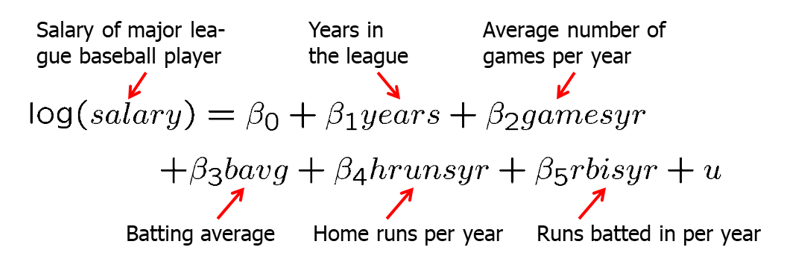
\includegraphics[width=0.8\textwidth]{figs/excl.png}
\end{figure}
\begin{itemize}
    \item $H_0:~\beta_3=0, \beta_4=0, \beta_5=0$ against $H_1:~H_0$ is not true

\item Test whether performance measures have no effect/can be excluded for the regression
\end{itemize}

}

\frame<beamer>{\frametitle{\textcolor{CUNEFOrange}{ Estimation of the unrestricted model
}}
\begin{figure}[htp]
    %\centering
    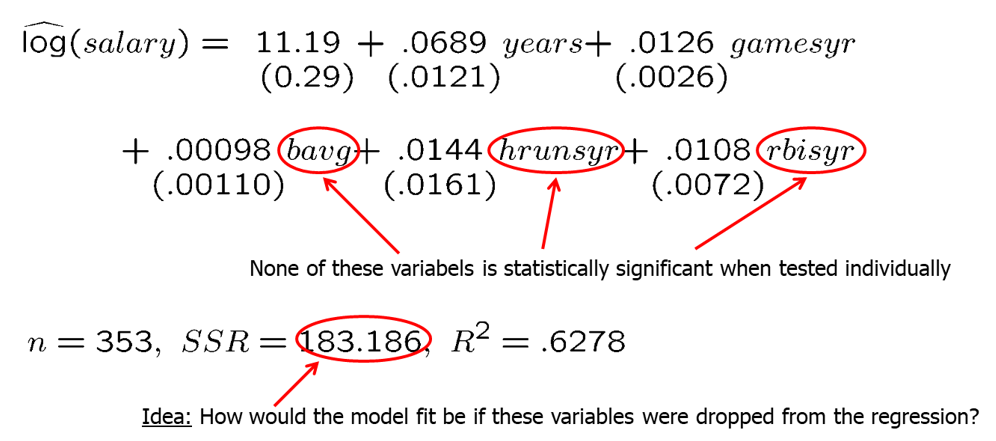
\includegraphics[width=0.9\textwidth]{figs/unrestr.png}
\end{figure}
}

\frame<beamer>{\frametitle{\textcolor{CUNEFOrange}{Estimation of the restricted model }}

\begin{figure}[htp]
    %\centering
    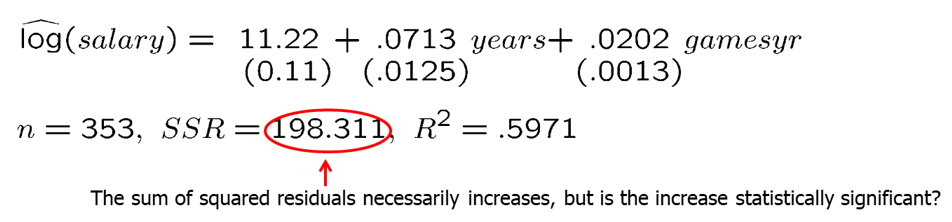
\includegraphics[width=0.8\textwidth]{figs/restr.png}
\end{figure}
\begin{itemize}
    \item Test statistic:
\[F=\frac{(SSR_r-SSR_{ur})/q}{SSR_{ur}/(n-k-1)}\sim F_{q,n-k-1}\]
\item $q$ is the number of restrictions
\item The relative increase of the sum of squared residuals when going from $H_1$ to $H_0$ follows a $F$-distribution (if the null hypothesis $H_0$ is correct)
\end{itemize}

}

\frame<beamer>{\frametitle{\textcolor{CUNEFOrange}{Rejection rule
 }}
\noindent
\begin{minipage}{.45\textwidth}
%\vspace{-1cm}
   \begin{figure}[h]
    %\centering
    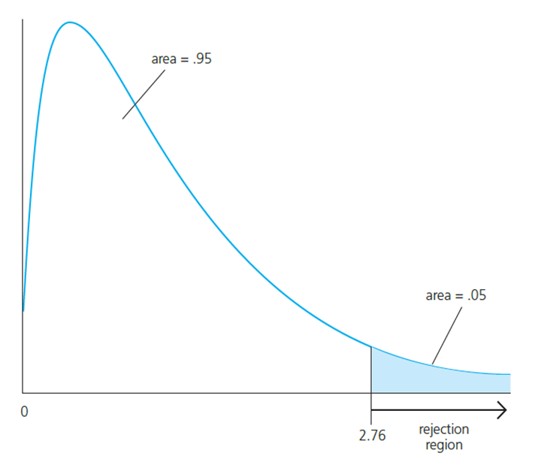
\includegraphics[width=1\textwidth]{figs/rej.png}
 \end{figure}
\end{minipage}%
\hspace{1cm} 
\begin{minipage}{.45\textwidth}
\vspace{0.5cm}

\begin{itemize}
\item A F-distributed variable only takes on positive values. This corresponds to the fact that the sum of squared residuals can only increase if one moves from $H_1$ to $H_0$.

\item Choose the critical value so that we incorrectly reject the null hypothesis in, for example, only 5\% of the cases.

\end{itemize} 
\end{minipage}
}

\frame<beamer>{\frametitle{\textcolor{CUNEFOrange}{Test decision in example
 }}

\begin{figure}[htp]
    %\centering
    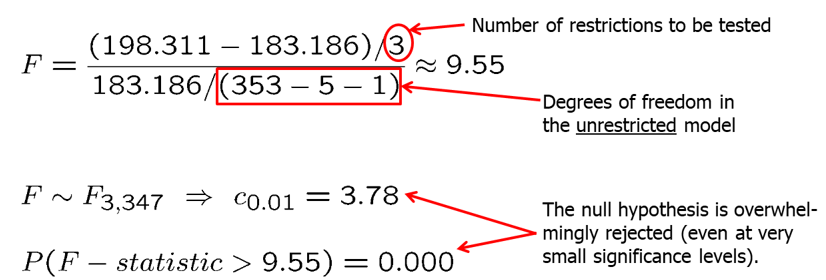
\includegraphics[width=0.8\textwidth]{figs/example_test.png}
\end{figure}
Discussion:
\begin{itemize}
    \item The three variables are “jointly significant”
\item They were not significant when tested individually
\item The likely reason is multicollinearity between them 
\end{itemize}

}


\frame<beamer>{\frametitle{\textcolor{CUNEFOrange}{Test of overall significance of a regression
 }}
\[y = \beta_0 +\beta_1 x_{i1}+\beta_2 x_{i2} + \ldots ++\beta_k x_{ik} +u\]
$H_0:~\beta_1=\beta_2=\ldots=\beta_k=0$ $\leftarrow$ The null hypothesis states that the explanatory variables are not useful at all in explaining the dependent variable
\[y = \beta_0+u \leftarrow \text{Restricted model (regression on constant)}\]
\[F=\frac{(SSR_r-SSR_{ur})/q}{SSR_{ur}/(n-k-1)} \]
%Discussion
%\begin{itemize}
%    \item The three variables are “jointly significant”
%\item They were not significant when tested individually
%\item The likely reason is multicollinearity between them 
%\end{itemize}

}

\frame<beamer>{\frametitle{\textcolor{CUNEFOrange}{ Testing general linear restrictions with the F-test
}}
Example: Test whether house price assessments are rational
\begin{figure}[htp]
    %\centering
    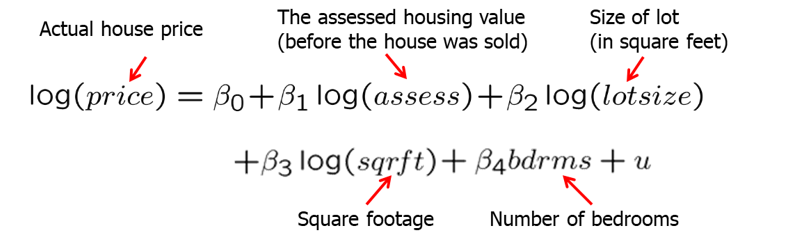
\includegraphics[width=0.8\textwidth]{figs/houseprice.png}
\end{figure}

\begin{itemize}
    \item $H_0:~\beta_1=1, \beta_2=0, \beta_3=0, \beta_4=0$
\item In addition, other known factors should not influence the price once the assessed value has been controlled for
\item If house price assessments are rational, a 1\% change in the assessment should be associated with a 1\% change in price
\end{itemize}

}

\frame<beamer>{\frametitle{\textcolor{CUNEFOrange}{ Testing general linear restrictions with the F-test (cont.)}}
\begin{itemize}
    \item Unrestricted regression
\[\text{log}(price)=\beta_0 +\text{log}(assess)+\beta_2\text{log}(lotsize)+\beta_3\text{log}(sqrft)+\beta_4 bdrms+u\]
\item Restricted regression
\[\text{log}(price)=\beta_0 +\text{log}(assess)+u\]
\[\text{log}(price)-\text{log}(assess)=\beta_0 +u\]
$\rightarrow$ The restricted model is actually a regression of $\text{log}(price)-\text{log}(assess)$ on a constant
\item Test statistic
\[F=\frac{(SSR_r-SSR_{ur})/q}{SSR_{ur}/(n-k-1)}=\frac{(1.880-1.822)/4}{1.822/(88-4-1)}\approx .661\]
$F\sim F_{4,83} \Rightarrow c_{0.05}=2.50 \Rightarrow H_0$ cannot be rejected
\end{itemize}

}

%%%%%%%%%%%%%%%%%%%%%
% Back Page
%%%%%%%%%%%%%%%%%%%%
\NoLogoFootline
{\usebackgroundtemplate{%

\includegraphics[width=\paperwidth,height=\paperheight]{figs/back_page.png}}
\slide{}{}}


\end{document}

\end{alertblock}
\begin{tcolorbox}[colback=white,colframe=CUNEFOrange,title=A nice heading]
some formula
\end{tcolorbox}
